\addcontentsline{toc}{chapter}{Summary}
\chapter*{Summary}
\setcounter{figure}{0}
\renewcommand\thefigure{\arabic{figure}}
\renewcommand\theequation{\arabic{figure}}
\ihead{Summary}

Particle physics studies the smallest building blocks that make up the world: the elementary particles.
Their size is orders of magnitude smaller than anything we encounter in daily life, even much smaller than biological cells.
The three particles making up atoms -- which we are all made of -- are the up and down~quarks, making up the protons and neutrons in the atomic nuclei, and the electrons circling around them.

An interesting phenomenon discovered in the first half of the previous century, is that of antimatter.
Antimatter particles behave exactly the same as the ordinary matter that we see around us, with two exceptions: their charge is inverted, and they only occur in nature in limited amounts.
Especially the latter is an interesting topic for research.
When we produce matter at large particle colliders, we always produce equal amounts of antimatter.
Taking this argument and applying it backwards in time, all the way to the origin of the universe, our universe should be filled with exactly the same amount of antimatter as matter!

But this is not the case.
We, our planet, our solar system, and all the stars and galaxies we can observe surrounding us, consist purely of matter.
The big question is then, where did the antimatter go?
The research in this thesis aims to improve our understanding of this very fundamental question.

\begin{figure}[htb] \centerfloat
    \begin{tikzpicture}
        \node[anchor=south west,inner sep=0] (image) at (0,0) {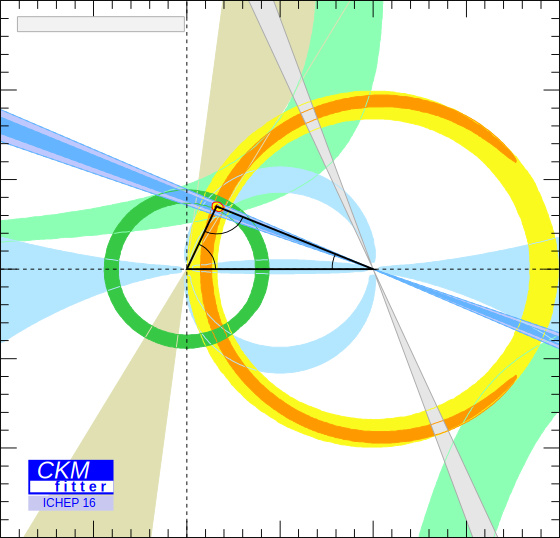
\includegraphics[width=0.55\textwidth]{theory/rhoeta_large}};
        \begin{scope}[x={(image.south east)},y={(image.north west)}]
            \node at (1. / 6. - 0.02, -0.027) {\(\pgfmathprintnumber[fixed,precision=1,fixed zerofill=true]{-0.5}\)};
            \foreach \x in {0, 2, 3, ..., 6}
            {
                \tikzmath{\xpos = \x / 6.; \xtext = \x * 0.5 - 1.0;}
                \node at (\xpos, -0.027) {\(\pgfmathprintnumber[fixed,precision=1,fixed zerofill=true]{\xtext}\)};
            }
            \node[anchor=east] at (0.005, 0.008) {\(\pgfmathprintnumber[fixed,precision=1,fixed zerofill=true]{-1.5}\)};
            \foreach \y in {1, ..., 6}
            {
                \tikzmath{\ypos = \y / 6.; \ytext = \y * 0.5 - 1.5;}
                \node[anchor=east] at (0.005, \ypos) {\(\pgfmathprintnumber[fixed,precision=1,fixed zerofill=true]{\ytext}\)};
            }

            {
                \fontsize{4}{4.8}\selectfont
                \node[anchor=west] at (0.04, 0.955) {excluded area has \({\text{CL} > \num{0.95}}\)};
                \node[anchor=west,rotate=-68] at (0.475, 0.995) {excluded at \({\text{CL} > \num{0.95}}\)};
                \node[anchor=west] at (0.76, 0.08) {sol. w/ \({\cos 2\CPbeta < 0}\)};
                \node[anchor=west] at (0.76, 0.05) {(excl. at \({\text{CL} > \num{0.95}}\))};
            }
            {
                \fontsize{10}{12}\selectfont
                \node[anchor=west] at (0.40, 0.885) {\CPgamma};
                \node[anchor=west] at (0.665, 0.810) {\dmd~\&~\dms};
                \node[anchor=west] at (0.02, 0.730) {\({\sin 2\CPbeta}\)};
                \node[anchor=west] at (0.82, 0.630) {\dmd};
                \node[anchor=west] at (0.03, 0.575) {\epsK};
            }
            {
                \fontsize{7}{8.4}\selectfont
                \node[anchor=west] at (0.365, 0.580) {\CPalpha};
                \node[anchor=west] at (0.530, 0.519) {\CPbeta};
                \node[anchor=west] at (0.34, 0.514) {\CPgamma};
            }
            {
                \fontsize{10}{12}\selectfont
                \node[anchor=west] at (0.03, 0.460) {\CPalpha};
                \node[anchor=west] at (0.175, 0.390) {\abs{\Vub}};
                \node[anchor=west] at (0.59, 0.390) {\CPalpha};
                \node[anchor=west] at (0.205, 0.165) {\CPgamma};
                \node[anchor=west] at (0.86, 0.190) {\epsK};
            }

            \node[anchor=east] at (1.0, -0.10) {\wolfrhob};
            \node[rotate=90,anchor=east,inner xsep=0pt,outer xsep=0pt] at (-0.12, 1.0) {\wolfetab};
        \end{scope}
    \end{tikzpicture}
    \caption{
        One of the so-called \emph{Unitarity Triangles} of the Standard~Model.
        Its surface area is a measure of the amount of \CP~violation in nature.
        The shaded areas each correspond to a different kind of measurement of \CP~violation, and the size of the area to the uncertainty on that measurement.
        The fact that they agree at the apex of the triangle indicates the validity of the SM.
        This thesis presents a measurement of the parameter~\CPgamma, the lower-left angle of the triangle.
        This parameter is one of the least-known parameters of the SM, as can also be seen from the fact that its corresponding shaded area is the largest of all parameters in the figure.}
    \label{fig:summary_UT}
\end{figure}
%
One explanation is that matter and antimatter behave similarly, but not exactly the same.
The violation of the symmetry between matter and antimatter is called \CP~violation, and a small amount of it is actually predicted by our current understanding of the laws of physics (see \cref{fig:summary_UT}).
However, the amount of \CP~violation that we observe in nature is nowhere close to the amount necessary to explain the abundance of matter in the universe.
And so, the question remains open: what happened to the antimatter?

\begin{figure}[htb] \centerfloat
    \hspace*{-.5cm}
    \begin{tikzpicture}[font=\captionfont]
        \node[anchor=south west,inner sep=0] (image) at (0,0) {\includegraphics[width=1.\textwidth]{detector/LHCb}};
        \begin{scope}[x={(image.south east)},y={(image.north west)}]
            \draw [very thick, ->] (-.1, .45) -- (.01, .45) node [at start,anchor=north west] {\normalsize \proton};
            \draw [very thick, ->] (.95, .45) -- (.84, .45) node [at start,anchor=north east] {\normalsize \proton};

            \draw [very thick] (.11, .47) -- (.11, 0.85) node [right,anchor=north west,inner ysep=0pt,outer sep=0pt] {\velo};
            \draw [very thick] (.16, .54) -- (.16, 0.80) node [right,anchor=north west,inner ysep=0pt,outer sep=0pt] {\rich~1};
            \draw [very thick] (.185,.48) -- (.185,0.75) node [right,anchor=north west,inner ysep=0pt,outer sep=0pt] {\ttracker};
            \draw [very thick] (.27, .65) -- (.27, 0.85) node [right,anchor=north west,inner ysep=0pt,outer sep=0pt] {Magnet};
            \draw [very thick] (.413,.57) -- (.413,0.85) node [right,anchor=north west,inner ysep=0pt,outer sep=0pt] {\intr~\&~\ot};
            \draw [very thick] (.46, .61) -- (.46, 0.78) node [right,anchor=north west,inner ysep=0pt,outer sep=0pt] {\rich~2};
            \draw [very thick] (.57, .61) -- (.57, 0.85) node [right,anchor=north west,inner ysep=0pt,outer sep=0pt] {\presh~\&~\ecal};
            \draw [very thick] (.62, .63) -- (.62, 0.78) node [right,anchor=north west,inner ysep=0pt,outer sep=0pt] {\hcal};
            \draw [very thick] (.75, .67) -- (.75, 0.85) node [right,anchor=north west,inner ysep=0pt,outer sep=0pt,align=left] {Muon\\stations};
        \end{scope}
    \end{tikzpicture}
    \caption{
        Cutout of the \lhcb~detector, with its various components indicated.
        The \({\proton\proton}\)~collisions occur on the left side of the figure, inside the~\velo.}
    \label{fig:summary_LHCb}
\end{figure}
%
The research described in this thesis aims to provide more insight in \CP~violation through the decay of strange beauty mesons: \Bs~mesons, and their antimatter counterparts \Bsb~mesons.
These particles can not be detected directly, rather, they decay into other particles.
The decay of interest here is one into two other particles (or decay products): a \Dsmp~meson and a kaon~\Kpm.
The decay products can be measured by a particle detector, in this case the \lhcb~detector (see \cref{fig:summary_LHCb}) at the Large Hadron Collider of~\cern, located in Geneva.
This detector is the size of a small building, and is situated \SI{80}{\metre}~beneath the surface.
Within the detector, protons from the~\lhc are collided, which are accelerated to over~\SI{99.999}{\percent} of the speed of light.
These collisions cause massive numbers of particles to be produced.
Among those particles are the \Bs~mesons on which the research in this thesis is based.

First of all, it is studied how often this specific decay of a \Bs~meson occurs, as a fraction of all possible decays of such a particle.
This number is called the branching fraction.
The branching fraction is calculated from the total number of observed \BsDsK~candidates in the detector, and the efficiency with which those are detected.
The latter is obtained by simulating \BsDsK~events.
This simulation includes the full proton-proton collision, particle decays, material interactions and detector response.
The result is that the decay \BsDsK~occurs in about~\num{2} out of every~\num{10000} \Bs~mesons, yielding a total of about five thousand reconstructable \BsDsK~events in the full data set.
These events can be seen as the large peak on the left-hand side of \cref{fig:summary_mass}.

The way \CP~violation can be measured from these decays is through an interesting feature of \Bs~mesons: during their (short) lifetime, they rapidly oscillate into their corresponding antimatter particle and back.
This phenomenon is called \emph{mixing}, and it only occurs in a few specific particle types.
\CP~violation may show up in mixing as an asymmetry between two similar processes: the mixing and subsequent decay of a meson, and the same process for the antimatter counterpart of that meson.
Therefore, studying the mixing and decay of \Bs~mesons can yield a measurement of the amount of \CP~violation.

In order to study mixing, it is necessary to know how long a meson lived before decaying, called its decay time.
This can be done using the known mass and calculated momentum of the meson, according to
%
\begin{equation} \tag{1} \label{eqn:summary_resolution}
    t = \dfrac{m \upDelta x}{\ptot} \rlap{,}
\end{equation}
%
where \(t\)~is the decay time, \(m\)~the meson mass, \(\upDelta x\)~its determined travelling distance, and \(\ptot\)~its momentum.
To correctly use this number, the error on the number must also be determined.
An initial estimate of the error can be calculated by propagating the known errors on the numbers on the left-hand side of \cref{eqn:summary_resolution}.
However, this estimate is known to underestimate the true error on the decay time.
Therefore, it must be calibrated.
%
\begin{figure}[hp] \centerfloat
    \begin{tikzpicture}[scale=0.7, every node/.style={scale=0.7}]
        \node[anchor=south west,inner sep=0] (image) at (0,0) {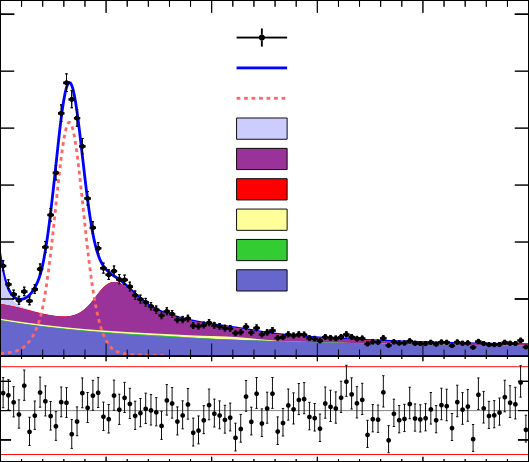
\includegraphics[width=0.9\textwidth]{BsDsK_TD/MDFit_Results/mass_Bs2DsK_BeautyMass_both_all_run1_nominal}};
        \begin{scope}[x={(image.south east)},y={(image.north west)}]
            \foreach \x/\xtext in {5300, 5400, ..., 5800}
            {
                \tikzmath{\xpos = (\x - 5300) / (5800 - 5300);}
                \node at (\xpos, -0.025) {\(\xtext\)};
            }
            \foreach \y in {0, ..., 6}
            {
                \tikzmath{\ypos = (\y / 6) * 0.740 + 0.217; \ytext = 200 * \y;}
                \node[anchor=base east] at (0.005, \ypos) {\(\pgfmathprintnumber[fixed,precision=0,fixed zerofill=true,1000 sep={}]{\ytext}\)};
            }
            \foreach \p in {0, ..., 2}
            {
                \tikzmath{\ypos = (\p / 2) * 0.127 + .048; \ptext = (\p - 1) * 2;}
                \node[anchor=east] at (0.005, \ypos) {\(\scriptstyle\pgfmathprintnumber[fixed,precision=0,fixed zerofill=true]{\ptext}\)};
            }
            \node[anchor=east] at (1.0, -0.09) {\({m(\DsmpKpm)}~[\si{\MeVcc}]\)};
            \node[rotate=90,anchor=east,inner xsep=0pt,outer xsep=0pt] at (-0.11, 1.0) {\({\text{Candidates}/(\SI{5.0}{\MeVcc})}\)};
            \node[anchor=west] at (0.06, 0.92) {\Huge\lhcb};
            % Legend
            {
                \node[anchor=base west] at (0.55, 0.906) {Data};
                \node[anchor=base west] at (0.55, 0.906 - 1 * 0.0656) {Total fit};
                \node[anchor=base west] at (0.55, 0.906 - 2 * 0.0656) {\BsDsK~signal};
                \node[anchor=base west] at (0.55, 0.906 - 3 * 0.0656) {\decay{\BorBsz}{\DsorDssmp\KorKstpm}};
                \node[anchor=base west] at (0.55, 0.906 - 4 * 0.0656) {\decay{\Bs}{\DsorDssm(\pip, \rhop)}};
                \node[anchor=base west] at (0.55, 0.906 - 5 * 0.0656) {\decay{\Bd}{\Dm(\pip, \Kp)}};
                \node[anchor=base west] at (0.55, 0.906 - 6 * 0.0656) {\LbDsOrDsstp};
                \node[anchor=base west] at (0.55, 0.906 - 7 * 0.0656) {\decay{\Lb}{\Lcp(\pim, \Km)}};
                \node[anchor=base west] at (0.55, 0.906 - 8 * 0.0656) {Combinatorial};
            }
        \end{scope}
    \end{tikzpicture}
    \caption{
        Distribution of the invariant mass of the combination of the \Dsmp~and \Kpm~mesons, as measured in the research described in this thesis.
        The dashed line on the left-hand side peaks at the mass of the \Bs~meson (about~\SI{5367}{\MeVcc}), and the events in that peak are the signal events of the decay~\BsDsK.
        The other events, shown as coloured areas, are background events and do not contribute to the measurement.}
    \label{fig:summary_mass}
\end{figure}
%
\begin{figure}[hp] \centerfloat
    \begin{tikzpicture}[scale=0.7, every node/.style={scale=0.7}]
        \node[anchor=south west,inner sep=0] (image) at (0,0) {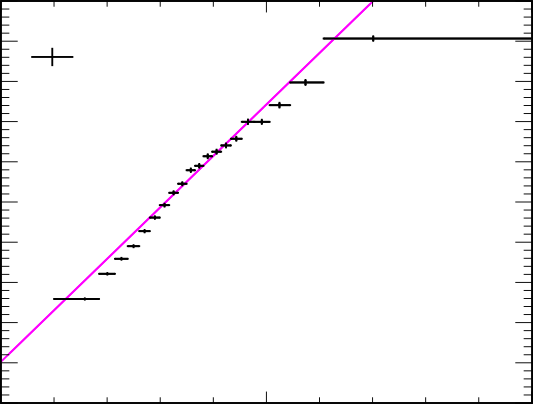
\includegraphics[width=0.9\textwidth]{summary/CombinationLinear_ALL_eff_sigma}};
        \begin{scope}[x={(image.south east)},y={(image.north west)}]
            \foreach \x in {0, ..., 10}
            {
                \tikzmath{\xpos = (\x / 10); \xtext = 10 * \x;}
                \node at (\xpos, -0.025) {\(\pgfmathprintnumber[fixed,precision=0,fixed zerofill=true]{\xtext}\)};
            }
            \foreach \y in {0, ..., 10}
            {
                \tikzmath{\ypos = (\y / 10); \ytext = 10 * \y;}
                \node[anchor=east] at (0.005, \ypos) {\(\pgfmathprintnumber[fixed,precision=0,fixed zerofill=true]{\ytext}\)};
            }
            % Legend
            {
                \node[anchor=base west] at (0.14, 0.843) {Prompt~\Dspm data};
            }
            \node[anchor=east] at (1.0, -0.09) {Initial decay-time error estimate~\([\si{\fs}]\)};
            \node[rotate=90,anchor=east,inner xsep=0pt,outer xsep=0pt] at (-0.12, 1.0) {Calibrated decay-time error~\({\sigma~[\si{\fs}]}\)};
        \end{scope}
    \end{tikzpicture}
    \caption{
        Decay-time error measured using prompt~\Dsmp events (black data points) as a function of the initial decay-time error estimate, and a linear fit to those points (solid line).
        This fit, with a slope of about~\num{1.3}, represents the scaling between the initial estimate and the real error on the decay time.}
    \label{fig:summary_resolution}
\end{figure}
%
This calibration must be done with events of which the decay time is already known.
In this case, a sample of prompt \Dsmp~events is used.
Each \Dsmp~meson is combined with a \Kpm~meson to obtain a combination that ``fakes'' a \Bs~meson: it looks like one, but its true decay time is known to be zero.
Hence, from the spread in observed decay time of those fake \Bs~mesons, the real error can be determined.
Comparing this to the initial estimate of the error yields a scaling, shown as the diagonal line in \cref{fig:summary_resolution}, which can be applied to real data to calibrate.

Using the decay times and calibrated decay-time errors, a measurement of \CP-violation can be extracted from the data.
This is done by \emph{tagging} the mesons: identifying whether they started out as a \Bs~meson or as the antimatter counterpart, a \Bsb~meson.
This yields four decay combinations to compare: a \Bs~or \Bsb~meson, either of which can decay into both final states~\DsmKp and~\DspKm.
In total, five \CP-violation parameters, called \Cpar, \Spar, \Sbpar, \Dpar, and~\Dbpar, are obtained by analysing the decay times of these four combinations.
These can be combined into a single measurement of the \CP-violation parameter~\CPgamma, first introduced in \cref{fig:summary_UT}.
This combination is illustrated in \cref{fig:summary_gamma}.

The result is~\({\CPgamma = \ang[parse-numbers=false]{\left(128_{-22}^{+17}\right)}}\), which significantly deviates from \ang[parse-numbers=false]{\left(0\!\mod 180\right)} and therefore represents the first evidence for \CP~violation in the decay channel~\BsDsK.
The value is higher than expected by about \num{2.3}~standard deviations with respect to the combination of other \lhcb~measurements of~\({\CPgamma = \ang[parse-numbers=false]{\left(72.2_{-7.3}^{+6.8}\right)}}\).
This deviation is small enough to be attributed to statistical fluctuations.
Nevertheless, it could also be a hint for new physics, such as a difference in \CP~violation in \Bp~meson decays, used mainly for the combined result, and in \Bs~mesons, used in the analysis presented in this thesis.
%
\begin{figure}[ht] \centerfloat
    \fontsize{18}{21.6}\selectfont
    \begin{tikzpicture}[scale=0.8, every node/.style={scale=0.8}]
        \node[anchor=south west,inner sep=0] (image) at (0,0) {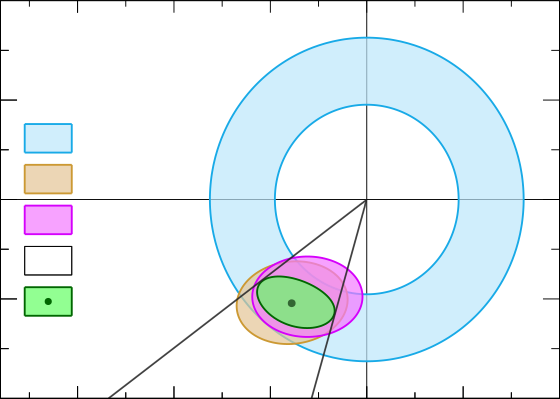
\includegraphics[width=0.9\textwidth]{Vub/Gamma/Lambda_f}};
        \begin{scope}[x={(image.south east)},y={(image.north west)}]
            \node at (0.139 + 0 * 0.172 - 0.02, -0.040) {\num{-1.5}};
            \node at (0.139 + 1 * 0.172 - 0.02, -0.040) {\num{-1}};
            \node at (0.139 + 2 * 0.172 - 0.02, -0.040) {\num{-0.5}};
            \node at (0.139 + 3 * 0.172, -0.040) {\num{0}};
            \node at (0.139 + 4 * 0.172, -0.040) {\num{0.5}};
            \node at (1.0, -0.040) {\num{1}};
            \node[anchor=east] at (0.005, 0.00) {\num{-1}};
            \node[anchor=east] at (0.005, 0.25) {\num{-0.5}};
            \node[anchor=east] at (0.005, 0.50) {\num{ 0}};
            \node[anchor=east] at (0.005, 0.75) {\num{ 0.5}};
            \node[anchor=east] at (0.005, 1.00) {\num{ 1}};

            % Legend
            {
                \fontsize{12}{14.4}\selectfont
                \node[anchor=base west] at (0.130, 0.640) {\(\sqrt{1 - \Cpar^{2}}\)};
                \node[anchor=base west] at (0.130, 0.640 - 1 * 0.103) {\({(-\Dpar, \Spar)}\)};
                \node[anchor=base west] at (0.130, 0.640 - 2 * 0.103) {\({(-\Dbpar, \Sbpar)}\)};
                \node[anchor=base west] at (0.130, 0.640 - 3 * 0.103) {\({-\left(\weak\right)}\)};
                \node[anchor=base west] at (0.130, 0.640 - 4 * 0.103) {Combination};
            }

            \node[anchor=east] at (1.0, -0.155) {\({\Im\left[2\lf / (1 + \abs{\lf}^{2})\right]}\)};
            \node[rotate=90,anchor=east,inner xsep=0pt,outer xsep=0pt] at (-0.14, 1.0) {\({\Re\left[2\lf / (1 + \abs{\lf}^{2})\right]}\)};
            \node[anchor=base west] at (0.06, 0.823) {\lhcb};
        \end{scope}
    \end{tikzpicture}
    \caption{
        Constraints imposed on the parameter~\CPgamma (black lines and green area) by the five \CP~violation parameters presented in this thesis (other shaded areas).
        The angle between the combination and the point~\({(0, 1)}\) implies a value of~\({\CPgamma = \ang[parse-numbers=false]{\left(\num{72.2}_{\num{-7.3}}^{+\num{6.8}}\right)}}\).}
    \label{fig:summary_gamma}
\end{figure}


